\documentclass[FM,MP]{tulthesis}  % Magisterský projekt fakulty mechatroniky
\usepackage[czech]{babel}  % Česká šablona dokumentu
\usepackage[utf8]{inputenc}  % Česká diakritika
\usepackage{graphicx}  % Tvorbě tabulek
\usepackage{float}  % Ukotvení věcí na svém místě (obrázky, tabulky, grafy, ...)
\usepackage{hyperref}  % Klikací odkazy v obsahu a referencích
\usepackage{gensymb}  % Pro stupne celsia
\usepackage{url}  % Pro lomeni adres url

\TULtitle{Zabezpečovací systém pomocí mobilního telefonu}{Security system using a mobile phone}
\TULprogramme{N2610}{Elektrotechnika a informatika}{Electrical Engineering and Informatics}
\TULbranch{1802T007}{Informační technologie}{Information Technology}
\TULauthor{Bc. Tomáš Moravec}
\TULsupervisor{doc. Ing. Josef Chaloupka, Ph.D.}
\TULyear{2017}

\begin{document}
\ThesisStart{male}

\begin{acknowledgement}
Děkuji vedoucí práce panu doc. Ing. Josefu Chaloupkovy, Ph.D. za odborné vedení a poskytnuté informace při zpracování magisterského projektu.
\end{acknowledgement}

% Abstrakt

\begin{abstractCZ}
Práce se zabývá problematikou zabezpečovacího systému, postaveného na platformě Arduino, řízeného z desktopové aplikace a s možností monitorování pomocí mobilní aplikace. Komunikace mezi zabezpečovacím systémem a mobilní aplikací má být realizována pomocí mobilního telefonu. V úvodu jsou definovány základní pojmy a požadované vlastnosti, na jejichž základě byly objednány jednotlivé komponenty. První část práce je věnována snaze o využití mobilního telefonu, jako prostředníka pro připojení do mobilní datové sítě. Tato cesta se ukázala jako slepá a byla tedy zvolena druhá alternativa, komunikace pomocí samostatného GPRS modulu. Výstupem práce je firmware, který řídí zabezpečovací systém a zajišťuje komunikaci, a desktopová aplikace pro úplné řízení zabezpečovacího systému. Poslední část, tedy mobilní aplikace zůstává nedokončená.

\end{abstractCZ}

\vspace{2cm}

\begin{abstractEN}

\end{abstractEN}

\tableofcontents
\clearpage

\begin{abbrList}
\textbf{SMS} & Short message service, služba krátkých textových zpráv\\
\textbf{GSM} & Groupe Spécial Mobile, globální systém pro mobilní komunikaci\\
\textbf{GPRS} & General Packet Radio Service, služba pro přenos dat v mobilní síti\\
\textbf{IDE} & Integrated development environment, integrované vývojové prostředí\\
\textbf{LED} & Light-Emitting Diode, dioda emitující světlo\\
\textbf{PIR} & Passive infrared sensor, infračervený sensor pohybu\\
\textbf{LAN} & Local Area Network, místní počítačová síť\\
\textbf{GBS} & Glass break detector, detektor rozbití skla\\
\textbf{API} & Application Programming Interface, rozhraní pro přístup k aplikaci\\
\textbf{USB} & Universal Serial Bus, univerzální sériová sběrnice\\
\end{abbrList}

% Úvod

\chapter{Úvod}
Téma bylo vypsáno doc. Ing. Josefem Chaloupkou, Ph.D. a zaujalo mne díky své tématické návaznosti na mou bakalářskou práci s názvem \uv{Koncept nízkonákladového sledovacího zařízení pro osobní automobily} \cite{Bachelor thesis}. V bakalářské práci jsem se věnoval vývoji sledovacího zařízení na založeného na platformě Arduino, které bylo komunikovalo pomocí SMS zpráv s mobilním telefonem. Dalším logickým krokem pro mne bylo, jak uvádím v závěru své bakalářské práce, řízení z desktopové aplikace, případně z mobilní aplikace, skrze mobilní datovou síť. Po konzultaci s vedoucím jsem byl obeznámen s tím, že tato práce mi nejen umožní navázat na předešlou práci bakalářskou, ale i prozkoumat možnosti využití starých, levných a nepoužívaných mobilních telefonů, jako náhradu za mnohdy drahé GPRS moduly. Nadchla mě myšlenka, že by bylo možné vzít starý nepoužívaný telefon, který má mnoho lidí ve vlastnictví, z důvodu neustálého obměňování za nejnovější modely, a nalézt pro něj smysluplné využití. Proto jsem se ihned přihlásil o toto zadání.

% Zabezpečovací systém
\chapter{Zabezpečovací systém}
Zabezpečovací systém, někdy také elektronická zabezpečovací signalizace, je zařízení, které vizuálně nebo akusticky vyhlašuje poplach a dává na vědomí, že nastaly nějaké potíže nebo došlo ke splnění sledované podmínky \cite{Security alarm}. Jde tedy o zařízení, které slouží k ochraně osob a majetku. Systém je řízen ústřednou a může se spustit analogovou (např. dveřní čidlo) i digitální (detektor pohybu) detekcí. Komunikace mezi detektory a ústřednou může být vedena kabelem, bezdrátově anebo kombinací předešlých způsobů, tj. jeden detektor může být připojen kabelem a druhý bezdrátově \cite{Electronic security system}.

\section{Ústředna}
Ústředna je „mozek“ celého systému, který je propojen s ostatními prvky systému kabely nebo bezdrátově. Obstarává komunikaci mezi jednotlivými komponenty systému, má v integrované paměti uložené nejdůležitější nastavení \cite{Electronic security system}. V závislosti na připojených komponentech pak může různě reagovat na splnění sledovaných podmínek. Často býva vybavena jenom tím nejnutnějším pro vyvolání poplachu, to ať už akustyckého (siréna), nebo tichého (informování majitele) \cite{Security alarm}.

\section{Ovladač}
Ovladač je prvek, který slouží k ovládání a případně též k programování ústředny. Dnešní alarmy je možné ovládat několika způsoby. Jako ovladač se nejčastěji používá klávesnice vybavená tlačítky, případně čtečkou (čipovými kartami a přívěšky) nebo též dálkové ovládání. U některých systémů se dá přes klávesnici provést nastavení celého systému. Klávesnice slouží k zastřežení i odstřežení systému \cite{Electronic security signalisation}. Dalšími způsoby je ovládání přes internet, kdy se většinou používá integrované webové rozhraní, ke kterému se uživatel může připojit po zadání hesla, nebo ovládání přes mobil (SMS příkazy) \cite{Bachelor thesis}.

\section{Detektor}
Detektor je prvkek systému, který je rozmístěn v hlídaném objektu a má za úkol reagovat aktivací při narušení (otevření, pohyb, rozbití atd.) a to tak, že tuto informaci předají ústředně, která ji následně zpracuje \cite{Electronic security signalisation}. Nejčastěji používané detektorové prvky jsou:

\begin{itemize}
\item Magnetický kontakt (dveřní čidlo)
\item Detektor pohybu (PIR detektor)
\item Detektor tříštění skla (GBS detektor)
\item Detektor plynu
\item Infra závora
\end{itemize} 

\section{Komunikátor}
Komunikátor je zařízení, které předává mimo objekt informaci o narušení objektu, případně o odchylce od normálního provozního stavu zabezpečovacího systému \cite{Electronic security signalisation}. Nejčastější typy komunikátorů jsou:

\begin{itemize}
\item GSM komunikátor
\item LAN komunikátor
\item Telefonní komunikátor
\item Komunikátor využívající radiové sítě s vyhrazenou frekvencí
\end{itemize} 

% Požadované vlastnosti a zvolené komponenty

\chapter{Požadované vlastnosti a zvolené komponenty}
V následující části se zaměřím na požadované vlastnosti zabezpečovacího zařízení a jaké komponenty byly na jejich základě zvoleny.

\section{Hardware}
Z úvodní části je jasné, že kompletní zabezpečovací systém musí obsahovat detektory, komunikátor a ústřednu. Rozebereme si tedy jednotlivé části.

\subsection{Ústředna}
Požadavky na ústřednu jsou takové, že musí být schopná komunikovat jak s desktopovou aplikací, tak s mobilní aplikací a zároveň musí řídit a zpracovávat jednotlivé komponenty. Zadání informuje o použití vývojové platformy Arduino, která je se svými periferiemi a čipem Atmega, více než vhodnou pro tyto účely. Firmware pro ústřednu bude psán v jazyku  C a C++ s nadstavbou Wiring (knihovny pro řízení hardwaru) \cite{Wiring}, vývojové prostředí Visual Studio 2017 s rozšířením Visual Micro \cite{Visual Micro}. Arduino Uno bylo zakoupeno v obchodu \url{arduino-shop.cz}.

\paragraph{Zvolená ústředna:}
\begin{itemize}
\item Arduino Uno Rev3 (700 Kč s DPH)
\end{itemize} 

\subsection{Detektory}
Požadavky nejsou kladeny pouze na samotné detektory, ale také na spínače, kterými bude možné spínat různá zařízení. Jako spínací prvky není nutné volit jednotlivé komponenty, stačí připravit implementaci jejich spínání. V případě detektorů musí být možné připojit libovolý detektor, který lze nastavit jako spínací (normálně rozepnutý), nebo rozpínací (normálně sepnutý). Pro testovací účely byly zvoleny dva detektory, každý jednoho typu. Sensor PIR byl objednán z číny.

\paragraph{Zvolené detektory:}
\begin{itemize}
\item Dveřní čidlo (rozpínací), (poskytl vedoucí)
\item PIR detektor (spínací), (25 Kč s DPH)
\end{itemize} 

\subsection{Komunikátor}
Požadavek na komunikátor je přenos dat do počítače a přes mobilní data. Zadání jako hlavní komunikátor určuje mobilní telefon, pomocí kterého máme umožnit ústředně datové přenosy. Zvolen byl nový a zároveň nejlevnější mobilní telefon na trhu, kteý byl zakoupen z obchodu Alza.cz. Pro případ neúspěchu, při získávání zdrojů mobilního telefonu, byla zvolena alternativa v podobě GSM/GPRS modulu, který byl zakoupen z Číny, dodací doba této součástky, stejně jako na všechny ostatní, byla přes jeden kalendářní měsíc.

\paragraph{Zvolené komunikátory:}
\begin{itemize}
\item Mobilní telefon STK R45i Black (449 Kč s DPH)
\item GSM/GPRS modul (290 Kč s DPH)
\end{itemize} 

\section{Software (Ovladač)}
Výše zmíněné prvky musí  být řízeny ovladačem, v mém případě aplikací jak desktopovou tak mobilní. Proto bude následující část rozdělena do těchto dvou částí.

\subsection{Desktopová aplikace}
Na desktopovou aplikaci jsou kladeny požadavky tak, aby byla schopna využít všech možností, které nám ústředna poskytuje. Musí být schopna kompletní správy a nastavení jednotlivých komponent (spínače a senzory) a tím pádem i komunikaci s ní. Cílový operační systém jsem si zvolil Windows 10, jakožto ve škole nejrozšířenější, programovací jazyk C\# a vývojové prostředí Visual Studio 2017. Jednotlivé požadavky kladené na desktopovou aplikaci lze nalézt níže.

\paragraph{Požadavky na desktopovou aplikaci:}
\begin{itemize}
\item Sledování aktuálních stavů komponent
\item Přidávání nových komponent
\item Odstraňování stávajících komponent
\item Přejmenování komponent
\item Změna pinů komponent
\item Změna nastavení senzorů jako spínacích či rozpínacích
\item Notifikace v případě změny stavů senzorů
\item Přepínání stavů spínačů
\item Připojování a odpojování ke zvolené ústředně
\end{itemize} 

\subsection{Mobilní aplikace}
Mobilní aplikace je učena pouze jako monitorovací zařízení, ze kterého bude možné sledovat stavy jednotlivých senzorů, případně spínač spínače. Její návrh je tedy značně jednodušší oproti komplexnější desktopové aplikaci. Cílový operační systém jsem zvolil Android, jakožto nerozšířenější, programovací jazyk Java a vývojové prostředí a Android Studio.

\paragraph{Požadavky na mobilní aplikaci:}
\begin{itemize}
\item Sledování aktuálních stavů komponent
\item Přepínání stavů spínačů
\item Připojování a odpojování ke zvolené ústředně
\end{itemize} 

% Hardware a firmware

\chapter{Hardware a firmware}

\section{Využití mobilního telefonu}
Následující část pojednává o snaze využít GSM/GPRS modulu integrovaném v mobilním telefonu. Práce na této části zabrali přibližně dva měsíce, proto bude rozdělena do více částí.

\subsection{Možné postupy}
První úkolem bylo, jak by bylo možné tyto zdroje z mobilního telefonu získat. Průzkumem existujících prací a internetu jsem mohl tento problém rozdělit na dvě kategorie. Chytré telefony a klasické telefony. U chytrých telefonů není získání těchto zdrojů problém, stačí napsat software, který tyto zdroje poskytne přes port USB a tím je problém vyřešen. Klasické telefony se dělí do dvou podkategorií. Telefony s dokumentací s API a poté telefon bez API a dokumentace. Některé starší telefony měli otevřené dokumentace a některá dokonce i API přímo pro tyto účely (Motorola, Nokia), pro tyto mobilní telefony existuje internet plný návodů jak se dostat ke zdrojům které chceme, nicméně takových modelů je opravdu malé množství. Poslední kategorií jsou mobilní telefony bez otevřených dokumentací a bez API, která by zpřístupňovala chtěné zdroje mobilního telefonu. Pro tyto mobilní telefony jsem nenalezl žádné dostupné řešení, přitom jsou to telefony nejrozšířenější a tím se staly pro tento projekt zajímavými.

\paragraph{Varianty telefonů:}
\begin{itemize}
\item Chytrý telefon (vyřešeno)
\item Klasický telefon s API (vyřešeno)
\item Klasický telefon bez API a dokumentace (nevyřešeno)
\end{itemize} 

\subsection{Výběr telefonu}
Prvním úkolem bylo vybrání vhodného kandidáta pro tyto účely. Nutné bylo tedy zvolit telefon pro které zatím není problém vyřešen. Po provedení průzkumu trhu jsem zjistil, že je možné vybírat jak z bazarových kousků, tak z nových. Zajimavým zjištěním bylo, že ceny nových telefonů podporujícíh s funkcí GSM i GPRS startují na 450 Kč s DPH za kus. Bazarové kousky začínají na 600 Kč s DPH za kus. Vzhledem k nižší ceně, záruce a garanci funkčnosti bylo rozhodnuto pro nový kus.

\subsection{První rozbor}
Před obdržením obdržení zakoupeného telefonu následoval průzkum, zda existují dokumentace, zda se někdo pokoušel alespoň o něco podobného a tak dále. Výsledkem bylo, že kromě oficiálního letáku s velice obecnými parametry přístroje, neexistují žádné veřejné dokumentace ani rozbory zařízení. Ihned po obdržení jsem se tedy pustil do vlastního průzkumu.

\begin{figure}[H]
\begin{center}
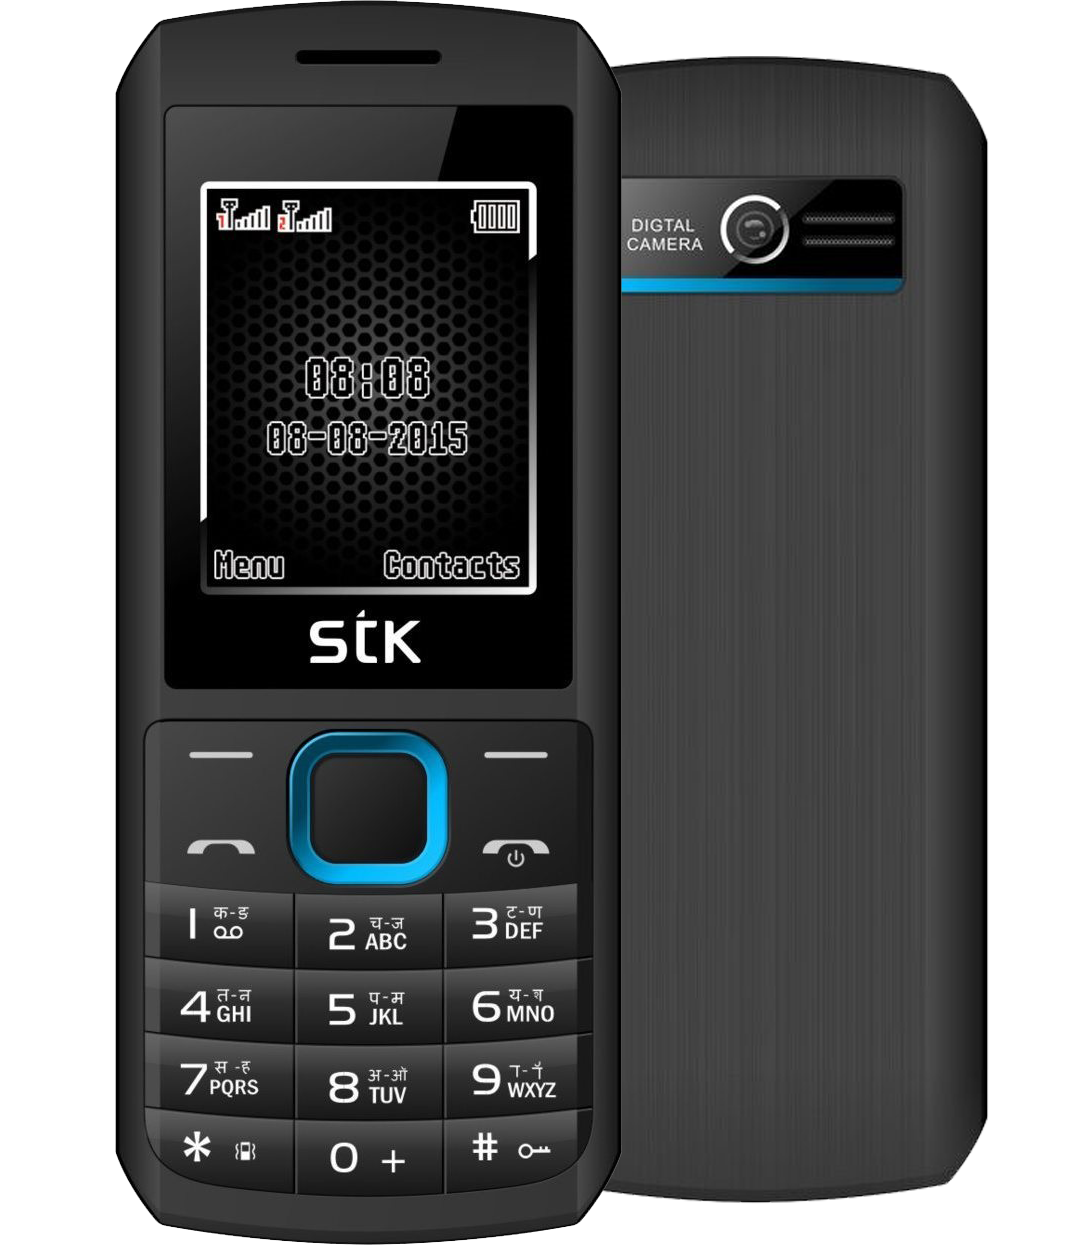
\includegraphics[width=0.4\textwidth]{images/phone.png}
\caption{Zakoupený mobilní telefon}
\label{image}
\end{center}
\end{figure}

\subsection{Kontaktování výrobce}
Jedním z prvních kroků bylo kontaktování výrobce s vysvětlením mého projektu a žádostí o poskytnutí dokumentačních podkladů. Napsal jsem celkem na 3 oddělení britské společnosti, přesněji na obchodní, podporu a servis. Mezitím jsem se pokusil o komunikaci s mobilním telefonem skrze USB, stejně jako to bylo možné u telefonů s API k těmto účelům, to se nepodařilo. Nakonec přišla schodná odpověď ze všech tří kontaktovaných oddělení, tedy že mi dokumentace neposkytnou.

\begin{figure}[H]
\begin{center}

\includegraphics[width=0.6\textwidth]{images/response.png}
\caption{Jednotná odpověď od společnosti STK}
\label{image}
\end{center}
\end{figure}

\subsection{Hlubší rozbor}
Bez dokumentací jsem musel začít zkoumat více do hloubky. Po konzultaci s vedoucím byl telefon rozebrán a zkoumán na případné servisní piny pro připojení a diagnostiku. Po hlubším prozkoumání se mi jako jednou variantu podařilo nalézt servisní piny, které jsem se následně snašil analyzovat a skrze ně komunikovat s mobilním telefonem.

\begin{figure}[H]
\begin{center}
\includegraphics[width=0.7\textwidth]{images/servicePins.png}
\caption{Objevené servisní piny}
\label{image}
\end{center}
\end{figure}

\subsection{Závěr rozboru}
Ani po několika týdenním snažení se nepodařilo z pinů dostat žádnou informaci. První týden se mi podařilo zachytávat neznámé signály, nicméně po hlubším přezkoumání spektráním analyzátorem bylo zjištěno, že se nejedná o číslicový signál. Po dvouměsíčním zkoumání jsem musel celou věc uzavřít a oznámit vedoucímu, že tudy zřejmě cesta nevede. Od této části projektu bylo tedy upuštěno.

\section{Zapojení}

\subsection{Blokové schéma}

\subsection{Výsledný prototyp}

\section{Firmware}

\subsection{Blokové schéma}

\subsection{Nastavení}

\subsection{API}

\subsection{Interní funkce}

\subsection{Notifikace}

% Desktopová aplikace

\chapter{Desktopová aplikace}

\subsection{Blokové schéma}

\subsection{Přehled}

\subsection{Nastavení sensoru}

\subsection{Nastavení spínače}

\subsection{Funkce programu a nastavení}

\subsection{Notifikace}

% Mobilní aplikace

\chapter{Mobilní aplikace}

% Závěr

\chapter{Závěr}

% Literatura

\addcontentsline{toc}{chapter}{Literatura}
\begin{thebibliography}{10}
\bibitem{Bachelor thesis}MORAVEC, Tomáš. Koncept nízkonákladového sledovacího zařízení pro osobní automobily: The concept of a low cost tracking device for personal cars. Liberec: Technická univerzita v Liberci, 2016.
\bibitem{Security alarm}Security alarm. Wikipedia [online]. [cit. 2017-05-23]. Dostupné z: \url{https://en.wikipedia.org/wiki/Security_alarm}
\bibitem{Electronic security system}Elektronické zabezpečovací systémy [online]. , 1 [cit. 2017-05-23]. Dostupné z: \url{http://www.ezasys.cz/elektronicke-zabezpecovaci-systemy/}
\bibitem{Electronic security signalisation}Elektronická zabezpečovací signalizace. Wikipedia [online]. [cit. 2017-05-23]. Dostupné z: \url{https://cs.wikipedia.org/wiki/Elektronick\%C3\%A1\_zabezpe\%C4\%8Dovac\%C3\%AD_signalizace}
\bibitem{Wiring}Wiring [online]. [cit. 2016-05-08]. Dostupné z: \url{http://wiring.org.co/}
\bibitem{Visual Micro}Visual Micro [online]. [cit. 2017-05-23]. Dostupné z: \url{http://www.visualmicro.com/}
\bibitem{Arduino intro}Arduino introduction. Arduino [online]. [cit. 2016-05-08]. Dostupné z: \url{https://www.arduino.cc/en/Guide/Introduction}
\bibitem{Arduino lib}Arduino libraries. Arduino [online]. [cit. 2016-05-08]. Dostupné z: \url{https://www.arduino.cc/en/Reference/Libraries}
\bibitem{Arduino lang}Arduino programming language. Arduino [online]. [cit. 2016-05-08]. Dostupné z: \url{https://www.arduino.cc/en/Reference/HomePage}
\bibitem{Arduino schematic}ARDUINO LLC. Arduino Schematic [online]. 1 s. [cit. 2016-05-07]. Dostupné z: \url{https://www.arduino.cc/en/uploads/Main/Arduino\_Uno\_Rev3-schematic.pdf}
\bibitem{Arduino soft} Arduino software. Arduino [online]. [cit. 2016-05-08]. Dostupné z: \url{https://www.arduino.cc/en/Main/Software}
\bibitem{Arduino source}Arduino source code. GitHub [online]. [cit. 2016-05-08]. Dostupné z: \url{https://github.com/arduino/Arduino/tree/1.6.8}
\bibitem{Atmega datasheet}ATMEL CORPORATION. ATmega48A/PA/88A/PA/168A/PA/328/P Datasheet [online]. 2015, 660 s. [cit. 2016-05-07]. Dostupné z: http://www.atmel.com/images/Atmel-8271-8-bit-AVR-Microcontroller-ATmega48A-48PA-88A-88PA-168A-168PA-328-328P\_ datasheet\_Complete.pdf
\bibitem{LaTeX}SATRAPA, Pavel. LaTeX pro pragmatiky [online]. 2011, 87 s. [cit. 2016-05-07]. Dostupné z: \url{http://www.nti.tul.cz/~satrapa/docs/latex/latex-pro-pragmatiky.pdf}
\bibitem{Pruvodce arduinem}VODA, Zbyšek. Průvodce světem Arduina [online]. Vydání první. Bučovice: Martin Stříž, 2015 [cit. 2016-05-07]. ISBN 978-80-87106-90-7.
\bibitem{SIMCOM SW}SIMCOM WIRELESS SOLUTIONS. SIM908 AT Command Manual [online]. Jinzhong, 2011, 249 s. [cit. 2016-05-07]. Dostupné z: \url{http://www.dfrobot.com/image/data/TEL0051/3.0/SIM908\_AT\%20Command\%20Manua\_V1.01.pdf}
\bibitem{SIMCOM HW}SIMCOM WIRELESS SOLUTIONS. SIM908 Hardware Design [online]. 2. Jinzhong, 2012, 53 s. [cit. 2016-05-07]. Dostupné z: \url{http://www.niplesoft.net/blog/wp-content/uploads/2016/02/SIM908-Hardware-Design-V2.00-1.pdf}
\bibitem{LaTeX}SATRAPA, Pavel. Stručný přehled příkazů LaTeXu [online]. 2011, 2 s. [cit. 2016-05-07]. Dostupné z: \url{http://www.nti.tul.cz/~satrapa/docs/latex/latex-prehled.pdf}
\end{thebibliography}

% Příloha

\appendix
\chapter{Obsah přiloženého CD}
Struktura a obsah adresářů je následující:

\paragraph{/Dokumentace}\mbox{}\\\mbox{}\\
Text bakalářské práce ve formátu pdf.

\paragraph{/Software}\mbox{}\\\mbox{}\\
Zdrojové kódy rozděleny do více kategorií.

\paragraph{/Software/Dokumentace (Datasheets)}\mbox{}\\\mbox{}\\
Softwarová a hardwarová dokumentace použitých součástek.

\paragraph{/Firmware/Firmware}\mbox{}\\\mbox{}\\
Hlavní software, nahraný ve sledovacím zařízení.

\end{document}